\documentclass[conference]{IEEEtran}
\usepackage{graphicx,booktabs,amsmath,url,array}
\usepackage{times}
\usepackage[hidelinks]{hyperref}
\graphicspath{{images/}}
\title{Calibration-Free P300 Decoding:\\Cross-Subject Transfer on BrainInvaders2013a}
\author{\IEEEauthorblockN{Birzhan Zhunusbekov, Arman Abakov, Nazerke Khamzina, Bekmurat Amangeldiyev}\IEEEauthorblockA{ROBT613 Midterm Project}}
\begin{document}
\maketitle
\begin{abstract}
We test whether a linear P300 decoder trained on other users can rank target flashes
above chance and how much it loses relative to subject-specific calibration.
The study uses 17 single-session BrainInvaders2013a subjects, two training runs per
subject, and a fixed five-channel physiological montage. A common pipeline extracts
50 ms ERP window means, scales features on training data, and fits shrinkage linear
discriminant analysis. Within-subject, leave-one-subject-out (LOSO), and class-count-matched
LOSO conditions share the same held-out test epochs. Mean subject-level ROC AUC is
0.875 $\pm$ 0.056 for Within, 0.724 $\pm$ 0.071 for LOSO-matched, and 0.810 $\pm$ 0.072 for LOSO.
Directional subject-level comparisons use Holm-adjusted Wilcoxon tests.
The study is retrospective and pilot-informed. It establishes offline flash-level
performance in this cohort, with no claim of online operation or exact permutation
inference for temporally dependent epochs.
\end{abstract}
\begin{IEEEkeywords}P300, EEG, cross-subject transfer, shrinkage LDA, grouped evaluation\end{IEEEkeywords}

\section{Question and Practical Significance}
A calibration phase asks a new BCI user to supply labelled examples before interaction.
Reducing that burden motivates generic decoders, but replacing a user's own data with
other people's recordings changes signal distributions. We ask whether a simple,
interpretable decoder still transfers when its preprocessing and feature representation
stay fixed. The question concerns the cost of transfer rather than the highest attainable
classification score.

Prior work motivates this question without supplying our numerical result. Barachant and
Congedo discuss generic initialization and continuing adaptation in a P300 system using
information geometry~\cite{barachant}. Kim and Kim report a zero-training system with a
pretrained xDAWN filter and convolutional network~\cite{kim}. Those methods provide
context only. Our core implementation uses the ERP and linear-classifier tools in
workshop notebooks 00--06~\cite{workshop}. We do not implement the later spatial or
nonlinear methods, and their device-control accuracy is not directly comparable to our
single-flash ROC AUC.

The original hypothesis has three parts. H1 states that LOSO AUC exceeds 0.5 on unseen
subjects. H2 states that Within exceeds LOSO on the same test runs. H3 states that Within
still exceeds LOSO when both training sets have the same class-specific epoch counts.
H3 addresses training-set size as an explanation for a transfer gap. It does not isolate
all physiological and recording differences between participants.

\subsection{Retrospective Development Boundary}
Subjects 8--10 informed the earlier development run. Before executing the full cohort,
we fixed a physiological montage of Cz, P3, Pz, P4 and Oz. The earlier implementation
pooled bad-channel flags over all subjects, allowing a held-out subject to affect the
training feature set. The revised implementation removes that dependency entirely.
It records the pooled flags for audit only. All three conditions use the same five
sites and 16 time windows, giving 80 features. This is a disclosed protocol revision,
not a claim of prospective preregistration. A sensitivity summary excludes the three
development subjects from evaluation.

\subsection{Study Logic}
Each of the 17 participants contributes two runs. One run tests and the other trains
the Within model. A LOSO model trains on both runs of all other participants and tests
on each of the held-out user's runs. A matched model uses a seeded subset of the same
external pool, with target and non-target counts equal to Within. Averaging ten matched
draws reduces dependence on a single random subset. The test epochs and outcome metric
remain identical across these conditions.

\clearpage
\section{Data Audit and Signal Inspection}
The acquisition report describes a visual P300 experiment recorded in 2013 with 16
scalp electrodes, a g.USBamp amplifier and a left-earlobe reference~\cite{vaineau}.
We retain subjects 8--24, who each have one session, to avoid the much larger download
for the longitudinal participants. This selection reflects protocol and compute
constraints rather than subject-level performance. It limits inference to this subset.
The notebook lists every subject ID explicitly.

\begin{table}[!ht]\centering\caption{Audited analysis contract}\small
\begin{tabular}{p{.39\columnwidth}p{.50\columnwidth}}\toprule
Property & Value\\\midrule
Subjects & 8--24 (17)\\
Sessions / runs & One / two per subject\\
EEG channels & 16 acquired; five decoder sites\\
Original sampling & 512 Hz\\
Analysis sampling & 128 Hz\\
MNE amplitudes & Volts; plots labelled in microvolts\\
Reference / ground & Left earlobe / Fz\\
Target / non-target code & 33285 / 33286\\
Flashes per original run & 80 target, 400 non-target\\
Total original flashes & 16320\\\bottomrule
\end{tabular}\end{table}

The audit confirms the expected sampling rate, channel count, conditions and class
counts for every included run. Run labels come from each subject's metadata, rather
than assuming a file number always identifies the same adaptive condition. Only the
training phases enter this analysis. The labels Adaptive and Non-Adaptive describe
the acquisition protocol; our offline LOSO model is not the original adaptive system.
\begin{figure}[!ht]\centering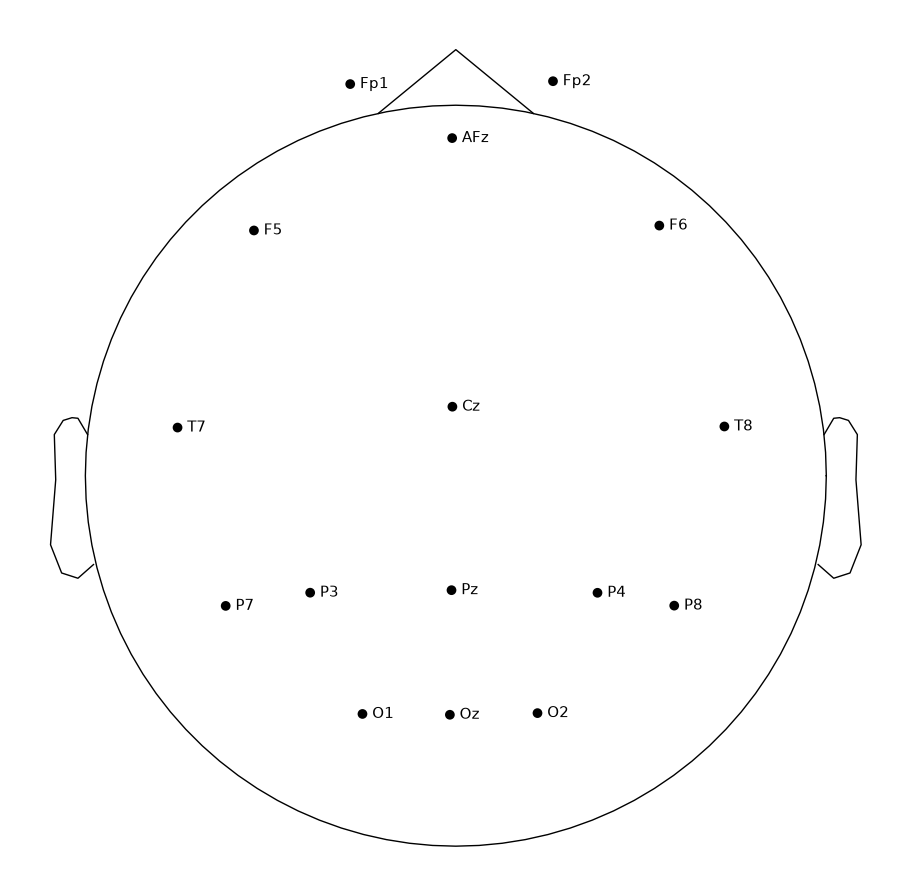
\includegraphics[width=\columnwidth]{images/sensors.png}\\\caption{Sensor layout from the MOABB/MNE montage. The decoder uses the fixed Cz/P3/Pz/P4/Oz subset. The remaining channels support inspection and artifact cleaning.}\end{figure}

\subsection{Acquisition and Download Provenance}
MOABB can prefer a mirror that provides only one training file. We therefore use the
original Zenodo archives and retrieve their metadata and training MAT members with
HTTP byte ranges. ZIP CRC checks verify archive-member extraction, and local SHA-256
manifests record the bytes. MOABB's original BI2013a reader still creates the MNE Raw
objects. The downloader changes file retrieval, not the EEG parser or event definitions.
Previously cached original files are reused. A server or network failure remains a
reproducibility constraint.

\subsection{Filtering and Sampling}
Every run is filtered separately with a zero-phase Hamming-window FIR band-pass from
0.5 to 20 Hz. The high-pass removes slow drift and the low-pass suppresses out-of-band
activity, including 50 Hz mains noise. A separate notch is omitted because the PSD and
residual line-noise measurements assess attenuation after the low-pass. The notebook
compares alternative high-pass cut-offs and a 30 Hz low-pass on the same example
flashes, so changes in retained trials do not masquerade as a filter effect.
\begin{figure}[!ht]\centering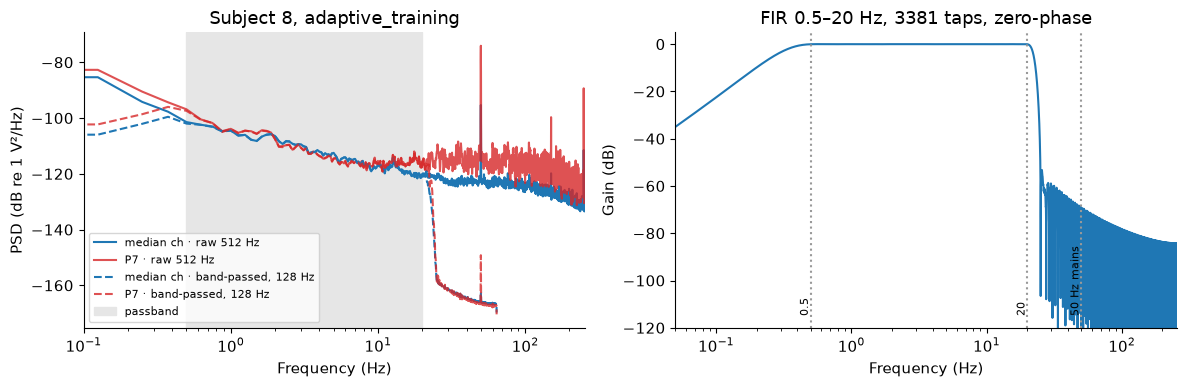
\includegraphics[width=\columnwidth]{images/psd.png}\\\caption{Example subject: Welch spectral inspection before and after preprocessing. The spectrum and the filter response motivate drift removal and a 20 Hz low-pass. This is evidence from the notebook, not a simulated signal.}\end{figure}

Resampling reduces 512 Hz to 128 Hz and resamples events together with the data.
The notebook reports timing differences and signal error. A recording-edge guard
uses the FIR half-support and the epoch bounds. It prevents the retained epochs from
using unsupported edge samples. No filter support crosses a run boundary. Zero-phase
filtering uses future samples, so the resulting system is explicitly offline.

\clearpage
\section{Artifact Handling and Neurophysiology}
Fp1 and Fp2 serve as ocular proxies because measured EOG is unavailable. These scalp
sites also contain neural activity, so proxy correlation cannot establish an exclusively
ocular source. The decoder excludes both sites.
\begin{figure}[!ht]\centering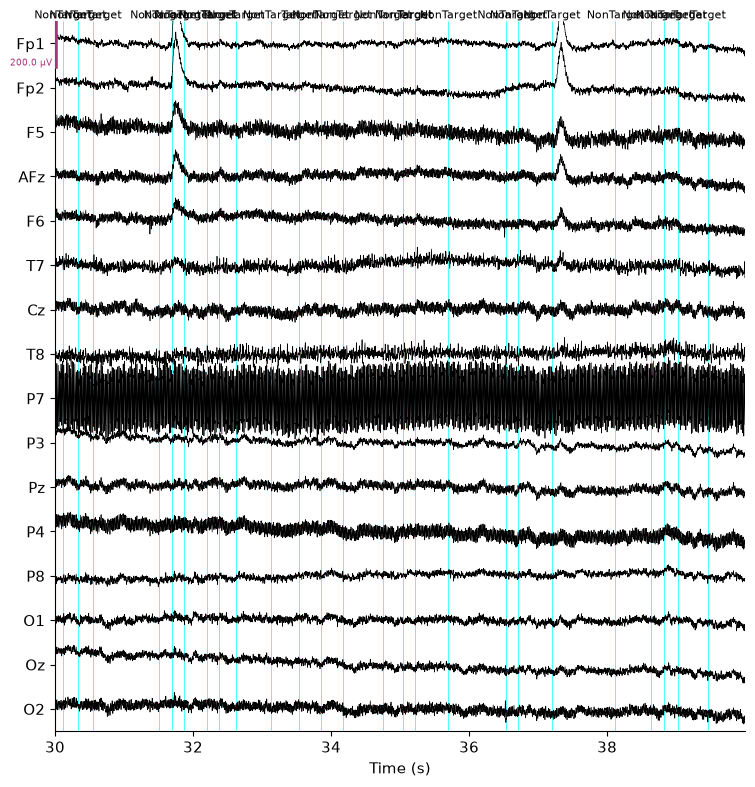
\includegraphics[width=\columnwidth]{images/raw.png}\\\caption{Unfiltered example EEG. The viewer removes display offsets. Large frontal transients motivate ocular-artifact handling; numerical data retain their original units.}\end{figure}

\subsection{Cleaning and Quality Control}
FastICA fits each unlabelled run on a 1--20 Hz copy at 128 Hz. The fitted unmixing
operator is then applied to the 0.5--20 Hz signal. Up to 15 components are retained,
with a reduction if flat channels reduce the available dimension. A component is
excluded only when the proxy-correlation outlier rule and a frontal-map-power rule
both flag it. Component evidence and before/after contrasts document the decision.

A channel is flat below 0.5 microvolt SD. A non-proxy channel is noisy when its cleaned
SD exceeds three times, or falls below one third of, the non-proxy median. Channels
remain visible in the audit. Runs with more than two bad channels and any flagged
core decoder site stop analysis for review. There is no interpolation and no pooled
channel-based feature selection.

Epochs extend from -100 to 800 ms. A 100 microvolt peak-to-peak rule rejects gross
residual artifacts after the edge guard. We report class-specific counts rather than
assuming rejection has no relation to target status. Across the full cohort, the edge
guard removes 3 targets and 12 non-targets. Amplitude rejection then
removes 80 targets and 329 non-targets. The analysis retains 2637
targets and 13259 non-targets, or 97.40 percent of all original flashes.

The baseline audit shows unequal preceding-flash class composition. Because responses
overlap, baseline subtraction could introduce a class-dependent offset. We use no
baseline subtraction in any condition.
\begin{figure}[!ht]\centering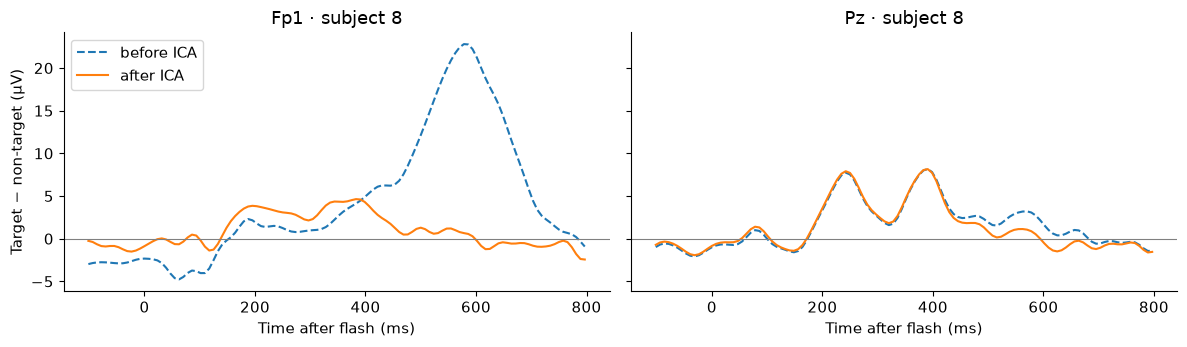
\includegraphics[width=\columnwidth]{images/artifacts.png}\\\caption{Example artifact contrast before and after ICA. Proxy channels support cleaning but do not enter the classifier. Residual artifacts remain a limitation.}\end{figure}

\subsection{Expected P300 Response}
Before decoding, target and non-target evoked responses are compared at Cz, Pz, P3,
P4 and Oz. The fixed Pz window is 250--600 ms. The full-cohort mean target-minus-non-target
window amplitude is 2.74 microvolts, with 16/17 subjects positive.
Peak amplitudes, latencies, single-trial images and scalp distributions supplement
the mean, so one number does not stand in for signal inspection.
\begin{figure}[!ht]\centering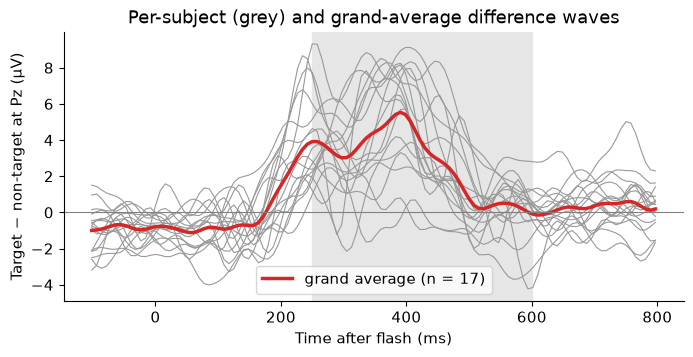
\includegraphics[width=\columnwidth]{images/group_wave.png}\\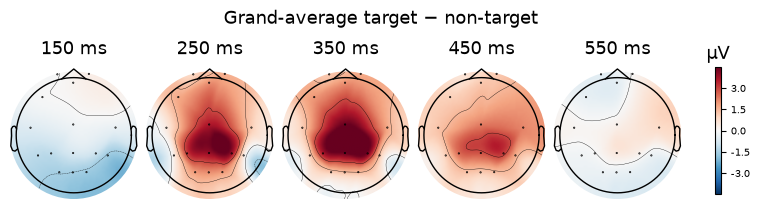
\includegraphics[width=\columnwidth]{images/group_erp.png}\\\caption{Group target-minus-non-target response and scalp distribution from the executed notebook. Each subject contributes equally to the grand average. The fixed Pz window is 250--600 ms.}\end{figure}

The response is consistent with P300 physiology. Cleaning does not establish neural
specificity: residual ocular activity and neighbouring responses may contribute.

\clearpage
\section{Features, Models and Honest Evaluation}
The feature map computes the mean amplitude in each of 16 consecutive 50 ms windows
between 0 and 800 ms at the fixed five sites. Each epoch becomes an 80-dimensional
vector. The window operation uses no estimated parameters or labels. It retains
ERP timing information without using CSP, xDAWN, wavelets, neural networks or other
methods outside the course's core scope.
\begin{figure}[!ht]\centering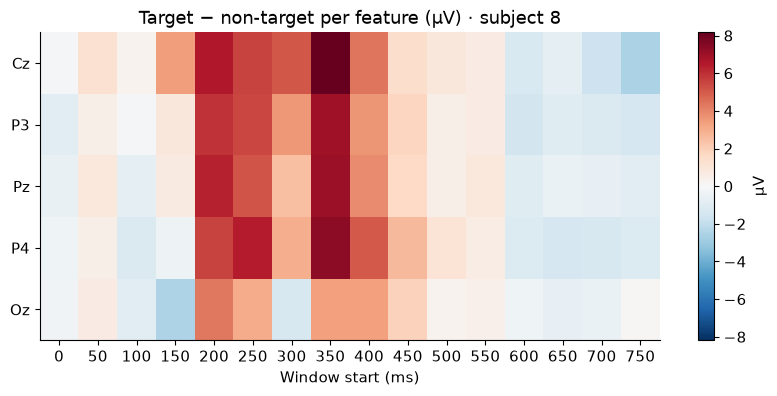
\includegraphics[width=\columnwidth]{images/features.png}\\\caption{Example subject: target-minus-non-target window means on the fixed five-channel montage. This descriptive heat map does not determine feature selection.}\end{figure}

\subsection{Training Boundary}
One scikit-learn Pipeline combines window means, StandardScaler and LDA with an
lsqr solver and analytic shrinkage. Scaling and covariance estimation fit only the
training set. No hyperparameter search uses test scores. In the transfer loop,
precomputing window means is equivalent to the stateless first Pipeline step; the
scaler and LDA still refit for each training set. An assertion checks that the Within
scores agree exactly with the separate grouped-CV implementation.

\begin{table}[!ht]\centering\caption{Controlled comparison for test run $r$ of subject $s$}\small
\begin{tabular}{p{.22\columnwidth}p{.66\columnwidth}}\toprule
Condition & Training observations\\\midrule
Within & Other run of $s$\\
LOSO & Both runs of every subject other than $s$\\
LOSO-matched & External epochs with Within's target and non-target counts; ten seeded draws\\\bottomrule
\end{tabular}\end{table}

Within evaluation uses LeaveOneGroupOut with run as the group. The transfer evaluation
leaves an entire subject out. No random epoch split is used, and no epoch from a test
subject enters the LOSO or matched training pool. Run-specific preprocessing keeps
samples from crossing the split, although unlabelled cleaning sees the complete test
run. The fixed montage ensures that test-subject channel flags cannot alter training.

\subsection{Metrics and Chance}
ROC AUC is primary because the original classes have a one-to-five ratio. AUC measures
target/non-target ranking and has a chance reference of 0.5. Balanced accuracy is also
reported for Within, using LDA's default decision rule without threshold tuning.
Mean and sample SD are reported across the two Within folds and across subject means.
These two kinds of spread answer different questions and must not be interchanged.

Within chance estimates use 200 label permutations restricted within run. LOSO chance
estimates shuffle held-out labels against a fixed score vector 1,000 times, avoiding
unnecessary refits. These shuffles retain class counts but do not preserve every
dependency in the flash sequence. Because epochs overlap, the resulting per-run
p-values are descriptive diagnostics rather than exact randomization inference.
Above-chance group evidence is assessed separately at subject level.

\subsection{Paired Statistical Comparison}
Each subject contributes its mean over the two held-out runs. The runs do not count
as independent people. H1 compares LOSO subject means with 0.5. H2 and H3 compare
paired subject means in the predicted direction. We report Wilcoxon p-values, median
paired differences and matched-pairs rank-biserial effects, excluding zero differences
from effect-size ranks. Holm correction covers the three primary hypotheses.
The LOSO-versus-matched comparison and ERP correlations remain exploratory.

A sensitivity analysis evaluates subjects 11--24 separately. Pilot subjects can still
appear in training pools for these new users, which is permitted for a generic decoder.
They do not contribute test outcomes to the sensitivity summary. This guards against
treating the development participants as wholly unseen evaluation cases.

\clearpage
\section{Full-Cohort Results}
Table~\ref{tab:subjects} gives the exact pairing underlying the hypothesis tests.
Across subject means, Within AUC is 0.875 $\pm$ 0.056, LOSO-matched is 0.724 $\pm$ 0.071, and
LOSO is 0.810 $\pm$ 0.072. These scores come from the executed notebook and exported CSVs.
The median Within-minus-LOSO gap is 0.072, compared with a median Within fold SD
of 0.018. The latter uses just two folds per subject and is an imprecise measure
of run variability.

\begin{table}[!ht]\centering\caption{Per-subject mean ROC AUC across two test runs}\label{tab:subjects}\small
\begin{tabular}{rrrr}\toprule
Subject & Within & Matched & LOSO\\\midrule
8 & 0.884 & 0.765 & 0.812 \\
9 & 0.883 & 0.821 & 0.906 \\
10 & 0.891 & 0.662 & 0.770 \\
11 & 0.913 & 0.721 & 0.777 \\
12 & 0.869 & 0.784 & 0.856 \\
13 & 0.861 & 0.652 & 0.738 \\
14 & 0.832 & 0.626 & 0.752 \\
15 & 0.929 & 0.700 & 0.862 \\
16 & 0.932 & 0.835 & 0.916 \\
17 & 0.812 & 0.609 & 0.671 \\
18 & 0.961 & 0.837 & 0.926 \\
19 & 0.805 & 0.663 & 0.714 \\
20 & 0.759 & 0.671 & 0.773 \\
21 & 0.960 & 0.758 & 0.848 \\
22 & 0.884 & 0.742 & 0.849 \\
23 & 0.882 & 0.737 & 0.789 \\
24 & 0.815 & 0.729 & 0.809 \\
\midrule
Mean & 0.875 & 0.724 & 0.810\\
SD & 0.056 & 0.071 & 0.072\\\bottomrule
\end{tabular}\end{table}

\begin{figure}[!ht]\centering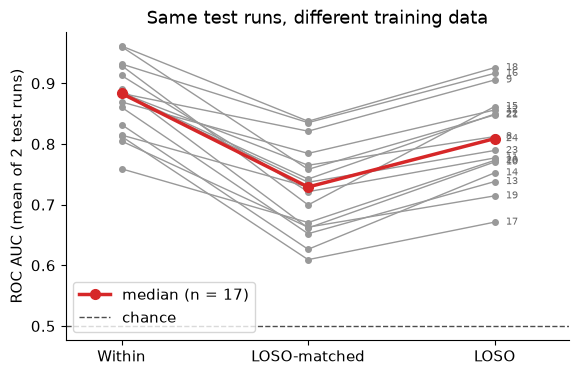
\includegraphics[width=\columnwidth]{images/comparison.png}\\\caption{Each line connects one subject across conditions. Test epochs are identical within a subject/run comparison. LOSO-matched averages ten class-count-matched draws.}\end{figure}

\begin{table}[!ht]\centering\caption{Primary tests: $n=17$ subject means}\small
\begin{tabular}{lrrrr}\toprule
Test & Median gap & $r_{rb}$ & Raw $p$ & Holm $p$\\\midrule
H1 & 0.309 & 1.000 & 7.6e-06 & 2.3e-05 \\
H2 & 0.072 & 0.895 & 0.00019 & 0.00019 \\
H3 & 0.142 & 1.000 & 7.6e-06 & 2.3e-05 \\
\bottomrule\end{tabular}\end{table}

Under the stated analysis, H1 is supported, H2 is supported, and H3 is supported.
The conclusions use adjusted p-values rather than selecting whichever unadjusted
comparison appears strongest. A supported directional difference would establish a
cohort-level ordering, not equivalence for every individual or a guaranteed benefit
for a future user. A non-significant comparison would indicate insufficient evidence
under this analysis, not proof of equal performance.

\begin{table}[!ht]\centering\caption{Sensitivity excluding development subjects from evaluation}\small
\begin{tabular}{lrrr}\toprule
Test & $n$ & Median gap & Holm $p$\\\midrule
H1 & 14 & 0.299 & 0.00018 \\
H2 & 14 & 0.073 & 0.00031 \\
H3 & 14 & 0.144 & 0.00018 \\
\bottomrule\end{tabular}\end{table}

The matched control addresses one practical alternative explanation. It preserves
Within's class-specific training counts, so an observed gap cannot be attributed only
to the total number of labelled epochs. The external examples come from several
participants, however, and thus also differ in diversity and dependence structure.
Ten draws quantify sampling variation, but do not remove those design differences.

\clearpage
\section{Interpretation, Limits and Reproducibility}
\subsection{What the Result Supports}
The main contribution is a controlled comparison with a common in-scope decoder,
identical test observations and explicit training boundaries. The full study extends
the pilot to the declared cohort and reports both individual outcomes and paired
comparisons. It asks how far a fixed linear ERP representation transfers, rather than
attributing a score change to simultaneous changes in classifier, preprocessing and
training quantity. The direction and magnitude of each result are reported even when
they do not meet a significance threshold.

The ERP-property plots explore why some users may be easier to decode. Amplitude,
latency and similarity to other users' grand average are measured descriptively.
Similarity uses only the other subjects to form its template. Nevertheless, these
associations use labelled test responses retrospectively, involve several comparisons,
and cannot guide a prospective decoder without a separate validation procedure.
\begin{figure}[!ht]\centering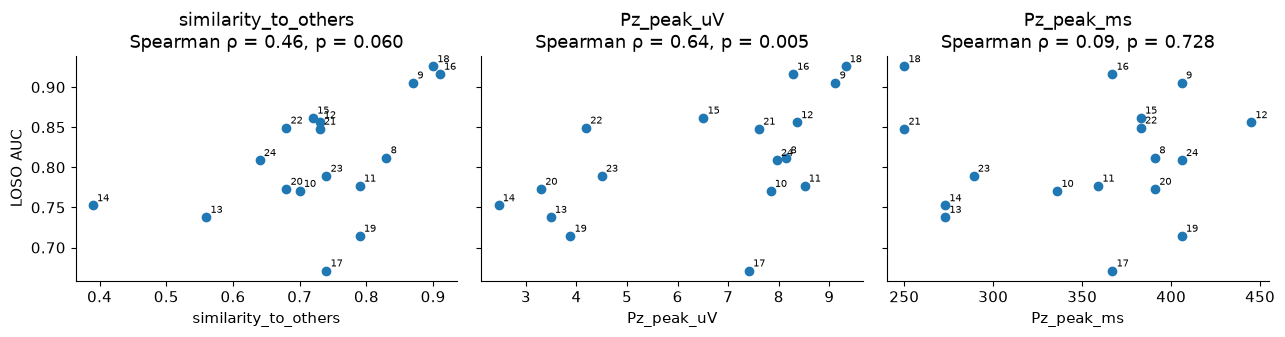
\includegraphics[width=\columnwidth]{images/exploratory.png}\\\caption{Exploratory relationships between LOSO AUC and ERP properties. These associations are descriptive and do not feed the decoder or establish causal mechanisms.}\end{figure}

\subsection{Limits}
The cohort includes 17 single-session users from one acquisition protocol. It does
not establish transfer to different equipment, clinical populations, days or tasks.
Both conditions are evaluated offline. Zero-phase filters and per-run ICA require
future unlabelled samples, and therefore cannot establish immediate plug-and-play
interaction. We decode single flashes rather than complete game commands. No character
accuracy, information-transfer rate or online device-control result follows from AUC.

Overlapping flashes weaken the exchangeability assumption behind unrestricted label
permutation. Subject-level comparisons reduce pseudoreplication, but the LOSO models
share training subjects, so fitted-model errors are dependent. We present Wilcoxon
statistics as conventional summaries of this fixed cohort, not exact guarantees for a
new population. Two runs also provide limited information about day-to-day stability.
Residual artifacts, pilot-informed decisions and the single physiological montage
remain further limits. A future preregistered study should lock choices on a separate
development cohort and test an independent acquisition.

\subsection{Execution and Versions}
Seed 613 and IDs 8--24 are explicit. The restarted Google Colab CPU session used Python 3.13.16. It completed in 7.41 minutes including setup checks and all data downloads; analysis after imports took 7.27 minutes. The dataset cache was initially empty. Pinned packages had been installed before a required NumPy restart. Request pacing and Retry-After handling resolved initial Zenodo rate limits. All notebook assertions passed. Saved notebook: \url{https://colab.research.google.com/drive/19qYoD5urhaAcdMhhokzYAZPZuN2ra2Rh}. CSVs and the manifest preserve exact results and versions.

\begin{table}[!ht]\centering\caption{Exact direct dependency versions}\small
\begin{tabular}{ll}\toprule
Package & Version\\\midrule
mne & 1.13.2 \\
moabb & 1.7.2 \\
numpy & 2.5.4 \\
scipy & 1.18.1 \\
pandas & 2.3.3 \\
scikit-learn & 1.9.1 \\
matplotlib & 3.11.2 \\
PyYAML & 6.0.3 \\
remotezip & 0.12.6 \\
threadpoolctl & 3.7.0 \\
\bottomrule\end{tabular}\end{table}

\subsection{Authorship}
The topic was registered on 15 October 2026. Lead and review roles and dated
contributions are recorded in the contribution log and the Git history submitted with
this report.

\subsection{Conclusion}
With fixed ERP features and a linear decoder, the full-cohort mean AUCs are 0.875 $\pm$ 0.056
for Within, 0.724 $\pm$ 0.071 for matched transfer and 0.810 $\pm$ 0.072 for LOSO. The primary
comparisons are H1: Holm $p=2.3e-05$; H2: Holm $p=0.00019$; H3: Holm $p=2.3e-05$. These results characterize offline transfer in this
cohort. They support discussion of calibration burden while preserving the limits of
a retrospective dataset analysis.

\appendices
\section{AI Tools Disclosure}
\textbf{OpenAI Codex} was used for code review, debugging, API lookup, implementation
changes to the notebook helpers, statistical checks, plotting, and drafting text for
the report and slides. \textbf{Claude Code} (Anthropic) was used to check the
submission against the assignment requirements and to edit report and README wording.
No AI tool generated results, citations or dataset facts: every number in this report
is exported from the executed notebook, and each citation was checked against its
source. All authors reviewed the submitted code and text and can explain it.

\clearpage
\begin{thebibliography}{9}
\bibitem{vaineau} E. Vaineau, A. Barachant, A. Andreev, P. Rodrigues, G. Cattan, and M. Congedo,
``Brain Invaders Adaptive versus Non-Adaptive P300 Brain-Computer Interface dataset,''
arXiv:1904.09111, 2019. \url{https://arxiv.org/abs/1904.09111}.
\bibitem{barachant} A. Barachant and M. Congedo, ``A Plug\&Play P300 BCI Using Information Geometry,''
arXiv:1409.0107, 2014. \url{https://arxiv.org/abs/1409.0107}.
\bibitem{kim} J. Kim and S.-P. Kim, ``A Plug-and-Play P300-Based BCI With Zero-Training Application,''
\emph{IEEE Trans. Neural Syst. Rehabil. Eng.}, vol. 33, pp. 3443--3454, 2025,
doi: 10.1109/TNSRE.2025.3603979.
\bibitem{workshop} B. Abibullaev, ``ROBT613 BCI Workshop: Brain--Computer Interfaces with
MNE-Python,'' notebooks 00--06, accessed Oct. 2026.
\url{https://berdakh.github.io/ROBT613-BCI-Workshop/},
\url{https://github.com/berdakh/ROBT613-BCI-Workshop}.
\bibitem{moabb} V. Jayaram and A. Barachant, ``MOABB: trustworthy algorithm benchmarking for BCIs,''
\emph{J. Neural Eng.}, vol. 15, no. 6, 066011, 2018.
\end{thebibliography}
\end{document}
